\documentclass[12pt]{article}

% This is the preamble, load any packages you're going to use here
\usepackage{physics} % provides lots of nice features and commands often used in physics, it also loads some other packages (like AMSmath)
\usepackage{siunitx} % typesets numbers with units very nicely
\usepackage{enumerate} % allows us to customize our lists
\usepackage[portuguese]{babel}
\usepackage{float} 
\usepackage{tabto}
\usepackage{graphicx}

\begin{document}

\title{Esvaziamento de tanques}
\author{Luiz Augusto Dembicki Fernandes}
\date{\today}

\maketitle

\begin{abstract}

\end{abstract}

\section{Montagem Experimental}

\tab  Foi mensurado o tempo(em triplicas) para dadas alturas em um tanque, utilizando diferentes bocais na saída do tanque, assim possibilitando avaliar seus efeitos no esvaziamento de um tanque.

\section{Dados}
Diametro do tanque: $ D_1 = 0,252m $ \\
Gravidade local: $ 9,78 m/s^2 $
\subsection[short]{Bocal 10mm}
$ k = 0,78 $
\begin{table}[H]
    \begin{tabular}{|l|lll|l|}
        \hline
        h(cm) & tempo                        &                              &       & Media de tempo \\ \hline
        40    & \multicolumn{1}{l|}{-}       & \multicolumn{1}{l|}{-}       & -     & -              \\ \hline
        35    & \multicolumn{1}{l|}{13,92}   & \multicolumn{1}{l|}{14,05}   & 13,83 & 00:00:13,93    \\ \hline
        30    & \multicolumn{1}{l|}{29,32}   & \multicolumn{1}{l|}{29,60}   & 29,47 & 00:00:29,46    \\ \hline
        25    & \multicolumn{1}{l|}{46,03}   & \multicolumn{1}{l|}{47,55}   & 46,51 & 00:00:46,70    \\ \hline
        20    & \multicolumn{1}{l|}{1:04,98} & \multicolumn{1}{l|}{1:04,94} & -     & 00:01:04,96    \\ \hline
        15    & \multicolumn{1}{l|}{1:26,15} & \multicolumn{1}{l|}{1:26,10} & -     & 00:01:26,13    \\ \hline
        10    & \multicolumn{1}{l|}{1:52,25} & \multicolumn{1}{l|}{1:51,23} & -     & 00:01:51,74    \\ \hline
        5     & \multicolumn{1}{l|}{2:10,85} & \multicolumn{1}{l|}{2:23,05} & -     & 00:02:16,95    \\ \hline
    \end{tabular}
    \caption{Bocal 10mm}
\end{table}

\subsection[short]{Bocal 7mm}
$ k = 0,78 $
\begin{table}[H]
    \begin{tabular}{|l|lll|l|}
        \hline
        h(cm) & tempo                            &                                  &             & Media de tempo \\ \hline
        40    & \multicolumn{1}{l|}{-}           & \multicolumn{1}{l|}{-}           & -           & -              \\ \hline
        35    & \multicolumn{1}{l|}{00:00:26,72} & \multicolumn{1}{l|}{00:00:27,62} & 00:00:27,62 & 00:00:27,32    \\ \hline
        30    & \multicolumn{1}{l|}{00:00:57,49} & \multicolumn{1}{l|}{00:00:57,74} & 00:00:57    & 00:00:57,42    \\ \hline
        25    & \multicolumn{1}{l|}{00:01:30,51} & \multicolumn{1}{l|}{00:01:31,71} & 00:01:30    & 00:01:31,06    \\ \hline
        20    & \multicolumn{1}{l|}{02:07,94}    & \multicolumn{1}{l|}{02:09,38}    & 00:02:08,19 & 00:02:08,50    \\ \hline
        15    & \multicolumn{1}{l|}{02:49,32}    & \multicolumn{1}{l|}{02:49,83}    & 00:02:49    & 00:02:49,47    \\ \hline
        10    & \multicolumn{1}{l|}{03:41,29}    & \multicolumn{1}{l|}{03:42,05}    & 00:03:41    & 00:03:41,46    \\ \hline
        5     & \multicolumn{1}{l|}{04:47,85}    & \multicolumn{1}{l|}{04:49,06}    & 00:04:47,70 & 00:04:48,20    \\ \hline
    \end{tabular}
    \caption{Bocal 7mm}
\end{table}

\subsection[short]{Bocal 4mm}
$ k = 0,78 $
\begin{table}[H]
    \begin{tabular}{|l|lll|l|}
        \hline
        h(cm) & tempo                            &                                  &             & Media de tempo \\ \hline
        40    & \multicolumn{1}{l|}{-}           & \multicolumn{1}{l|}{-}           & -           & -              \\ \hline
        35    & \multicolumn{1}{l|}{00:01:35,93} & \multicolumn{1}{l|}{00:01:35,59} & 00:01:35,66 & 00:01:35,73    \\ \hline
        30    & \multicolumn{1}{l|}{00:03:24,13} & \multicolumn{1}{l|}{00:03:23,63} & 00:03:23,89 & 00:03:23,88    \\ \hline
        25    & \multicolumn{1}{l|}{05:20,92}    & \multicolumn{1}{l|}{00:05:20,54} & -           & 00:05:20,73    \\ \hline
        20    & \multicolumn{1}{l|}{07:52,35}    & \multicolumn{1}{l|}{00:07:32,69} & -           & 00:07:42,52    \\ \hline
        15    & \multicolumn{1}{l|}{10:00,06}    & \multicolumn{1}{l|}{00:09:58,89} & 00:10:01,26 & 00:10:00,07    \\ \hline
        10    & \multicolumn{1}{l|}{12:53,53}    & \multicolumn{1}{l|}{00:12:52,48} & -           & 00:12:53,01    \\ \hline
        5     & \multicolumn{1}{l|}{16:30,53}    & \multicolumn{1}{l|}{00:16:30,15} & 00:16:30,80 & 00:16:30,49    \\ \hline
    \end{tabular}
    \caption{Bocal 4mm}
\end{table}

\subsection[short]{Sem Bocal 21mm}
$ k = 0,5 $
\begin{table}[H]
    \begin{tabular}{|l|lll|l|}
        \hline
        h(cm) & tempo                            &                                  &             & Media de tempo \\ \hline
        40    & \multicolumn{1}{l|}{-}           & \multicolumn{1}{l|}{-}           & -           & -              \\ \hline
        35    & \multicolumn{1}{l|}{00:00:03,88} & \multicolumn{1}{l|}{00:00:03,88} & 00:00:03,90 & 00:00:03,89    \\ \hline
        30    & \multicolumn{1}{l|}{00:00:07,78} & \multicolumn{1}{l|}{00:00:07,82} & 00:00:07,79 & 00:00:07,80    \\ \hline
        25    & \multicolumn{1}{l|}{00:00:12,01} & \multicolumn{1}{l|}{00:00:12,08} & 00:00:12    & 00:00:12,01    \\ \hline
        20    & \multicolumn{1}{l|}{00:00:16,55} & \multicolumn{1}{l|}{00:00:16,65} & 00:00:17    & 00:00:16,68    \\ \hline
        15    & \multicolumn{1}{l|}{00:00:22,05} & \multicolumn{1}{l|}{00:00:22,15} & 00:00:22    & 00:00:22,10    \\ \hline
        10    & \multicolumn{1}{l|}{00:00:27,94} & \multicolumn{1}{l|}{00:00:28,02} & 00:00:28    & 00:00:27,99    \\ \hline
        5     & \multicolumn{1}{l|}{00:00:35,77} & \multicolumn{1}{l|}{00:00:35,89} & 00:00:36    & 00:00:35,87    \\ \hline
    \end{tabular}
    \caption{Sem Bocal 21mm}
\end{table}


\section{Análise de dados}
Here you discuss your observations and results.

\subsection{Solução téorica}
\tab A solução téorica é resolvida utilizando o PVI:
\begin{center}
    $ \frac{dh(t)}{dt} =  -(\frac{r_2^2}{r_1^2}\cdot\sqrt{\frac{2g}{1 + k} } ) \sqrt{h(t)}$ ; $ h(0) = h_0 $
\end{center}
Utilizando $ h(0) = 0,4m$ e que o termo $(\frac{r_2^2}{r_1^2}\cdot\sqrt{\frac{2g}{1 + k} } ) = c$, temos que:
\begin{center}
    $ h(t) =  0,25 \cdot c^2  \cdot t^2 - (\frac{1}{2} \cdot 0,4m \cdot \sqrt{10})\cdot c   \cdot t + 0,4m$
\end{center}
Para cada diametro de bocal temos os seguintes valores de C:
\begin{table}[H]
    \begin{tabular}{|l|l|}
        \hline
        Bocal & C          $(m^2/s)$ \\ \hline
        10mm  & $5,220\cdot10^{-3}$  \\ \hline
        7mm   & $2,558\cdot10^{-3}$  \\ \hline
        4mm   & $8,352\cdot10^{-4}$  \\ \hline
        21mm  & $0,0251$             \\ \hline
    \end{tabular}
\end{table}
\subsection{Experimental}
\tab Foram então relacionados os respectivos tempos e alturas, teóricos e experimentais. Resultando nos seguintes gráficos:
\begin{center}

    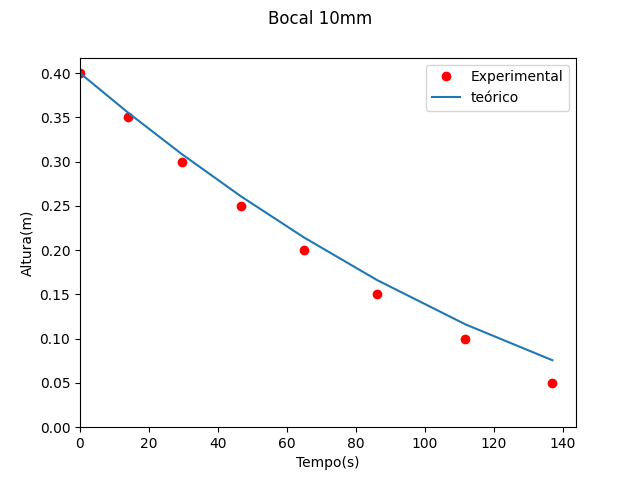
\includegraphics{bocal10.png}

    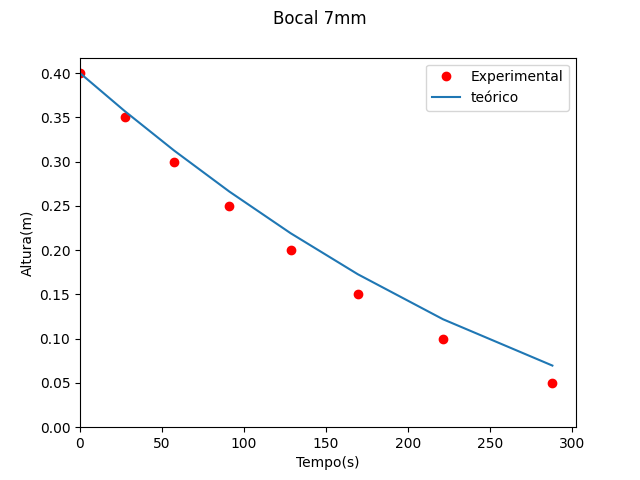
\includegraphics{bocal7.png}

    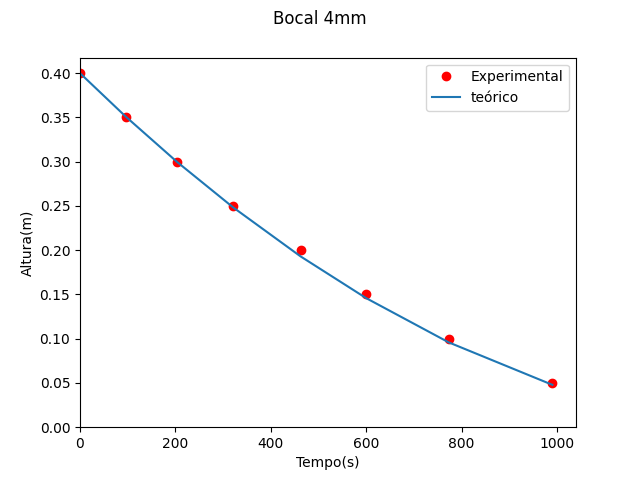
\includegraphics{bocal4.png}

    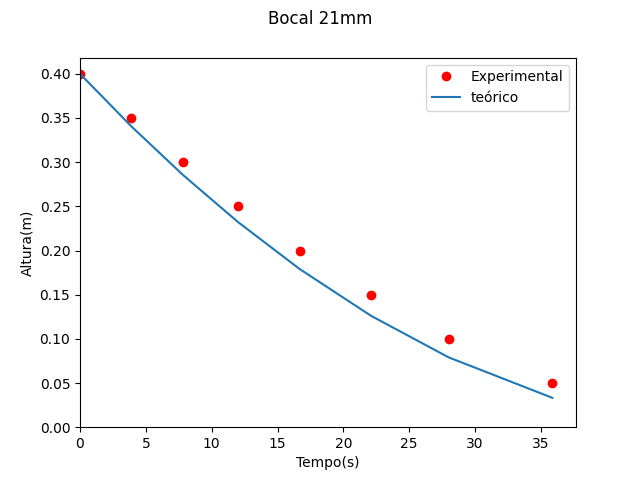
\includegraphics{bocal21.png}

\end{center}


\section{Conclusão}

\tab O resultado final está dentro do esperado para a prática. Os devios são mínimos o suficiente para se atribuir a algumas tomadas de tempo faltando.


\end{document}
